\documentclass[prl,aps,10pt,superscriptaddress,floatfix]{revtex4-2}
\usepackage[T1]{fontenc}
\usepackage{amsmath, amssymb, amsthm, mathtools, bbm}
\usepackage{dsfont}
\usepackage[dvipsnames]{xcolor}
\usepackage[colorlinks=true, pdfborder={0 0 0}]{hyperref}
\definecolor{googleblue}{RGB}{34, 0, 204}
\definecolor{panblue}{RGB}{0,24,150}
\definecolor{carmine}{RGB}{150, 0, 24}
\hypersetup{
unicode=true,
bookmarksnumbered=false,
bookmarksopen=false,
breaklinks=false,
colorlinks=true,
linkcolor=carmine,
citecolor=googleblue,
urlcolor=panblue,
anchorcolor=OliveGreen}

\usepackage{newtxtext}

\usepackage{tikz}
\usetikzlibrary{calc, arrows, patterns, shapes, decorations, arrows.meta, fit, positioning}
\usetikzlibrary{decorations.markings}
\tikzset{mid arrow/.style={postaction={decorate,decoration={markings,mark=at position 0.55 with {\arrow{Latex[length=4pt]}}}}}}

% Theorem environments
\newtheorem{theo}{Theorem}
\newtheorem{lemma}{Lemma}
\newtheorem{prop}{Proposition}
\newtheorem{coro}{Corollary}
\newtheorem*{defi}{Definition}
\newtheorem{obs}{Observation}

\begin{document}
\title{Generalized Probabilistic Topological Field Theories: Summary}
\author{Pedro Lauand}
\email{plauand@perimeterinstitute.ca}
\affiliation{Perimeter Institute for Theoretical Physics, Waterloo, Ontario, Canada, N2L 2Y5}

\begin{abstract}
Conceptual skeleton of the GPTFT program: the spacetime axioms, topological field theories as finite algebraic data, the category of GPTs as $\mathbf{Vec}$ plus positivity, the $1$d case as dualizability, and the $2$d case as a commutative Frobenius algebra whose finite data are positive GPT data.
\end{abstract}

\maketitle

\section{The spacetime axioms}\label{sec:intro}

\begin{itemize}
\item A field theory assigns: space $\to$ system, spacetime $\to$ process.
\item Locality is the compatibility of these assignments:
\[
Z(M'\circ M)=Z(M')\circ Z(M),\qquad
Z(\Sigma\sqcup\Sigma')=Z(\Sigma)\otimes Z(\Sigma').
\]
Gluing $\to$ composition (temporal locality); disjoint union $\to$ joint system (spatial locality).
\item Axioms (Atiyah--Segal \cite{Atiyah1988,Segal2004}): a field theory is a symmetric monoidal functor
\[
Z:\mathbf{Bord}_n\longrightarrow\mathcal C .
\]
\item The source is a choice of what spacetime is: in a \emph{topological} theory, bordisms up to diffeomorphism --- no metric, no local excitations.
\item The target is a choice of what physics is: $\mathbf{Vec}$, $\mathbf{Hilb}$ encode the linear skeleton of quantum theory; a \emph{GPT} target encodes directly the operational, probabilistic content \cite{Hardy2001,Barrett2007,Mueller2021,Plavala2023}.
\item \textbf{GPTFT} $:=$ TFT valued in the category of GPTs. Question: \emph{which probabilistic theories admit one?}
\end{itemize}

\section{Topological field theories}\label{sec:tft}

\begin{itemize}
\item $\mathbf{Bord}_n$: objects $=$ closed oriented $(n-1)$-manifolds; morphisms $=$ compact oriented $n$-bordisms up to diffeomorphism rel boundary; composition $=$ gluing; $(\sqcup,\varnothing)$ the monoidal structure.
\item Diffeomorphism invariance $\Rightarrow$ every manifold decomposes into finitely many elementary pieces $\Rightarrow$ a TFT is \emph{finite algebraic data} in $\mathcal C$: values on generators, subject to the relations identifying different decompositions of the same manifold.
\item $d=1$: generators interval, cup, cap; relations the snakes; a theory $=$ a \emph{dualizable object} of $\mathcal C$ (cobordism hypothesis \cite{Lurie2009}).
\item $d=2$: generators disk, pants, copants, reversed disk; a theory $=$ a \emph{commutative Frobenius algebra} in $\mathcal C$ \cite{Dijkgraaf1989,Abrams1996,Kock2004}.
\item Closed manifolds $\to$ endomorphisms of $\mathbf 1$, i.e.\ scalars: the \emph{invariants} of the theory.
\end{itemize}

\section{The category of GPTs: Vec plus positivity}\label{sec:gpt}

$\mathbf{Vec}$ (finite-dimensional real): all linear maps, monoidal product $\otimes$, compact closed --- duals, $\operatorname{ev}$, $\operatorname{coev}$ canonical, snakes automatic. GPT is the same data with one positivity condition per layer:
\[
\begin{aligned}
V\ &\rightsquigarrow\ (V,\,V^+,\,u),\\[2pt]
f\ &\rightsquigarrow\ f\ \ \text{with}\ \ f(V_A^+)\subseteq V_B^+,\\[2pt]
V_A\otimes V_B\ &\rightsquigarrow\ V_{AB}^+\in[\otimes_{\min},\otimes_{\max}],\quad u_A\otimes u_B.
\end{aligned}
\]

\begin{itemize}
\item \emph{Objects}: systems $A=(V_A,V_A^+,u_A)$; $V_A^+$ a proper cone of unnormalized states, $u_A\in V_A^*$ strictly positive on it. Normalized states $\Omega_A=u_A^{-1}(1)\cap V_A^+$; effects in the dual cone $(V_A^+)^*$; allowed effects $[0,u_A]$; measurements $(e_i)$, $\sum_ie_i=u_A$. No-restriction by default.
\item \emph{Morphisms}: cone-preserving linear maps. $\operatorname{Hom}_{\mathrm{GPT}}(A,B)$ is a \emph{cone}, not a subspace; GPT is a wide, non-full subcategory of $\mathbf{Vec}$. States and effects are arrows $\mathbf 1\to A$, $A\to\mathbf 1$; probabilities are composites $e\circ f\circ\omega\in\operatorname{End}(\mathbf 1)=\mathbb{R}$.
\item \emph{Composites}: underlying space $V_A\otimes V_B$ (tomographic locality), unit $u_A\otimes u_B$, composite cone any proper cone in $[\otimes_{\min},\otimes_{\max}]$. The interval collapses iff one factor is classical \cite{ALPP2021}; the quantum cone sits strictly between.
\item \emph{Departure from $\mathbf{Vec}$}: duals survive on objects ($X^\vee$ swaps state and effect cones onto $V^*$), but $\operatorname{ev}$ and $\operatorname{coev}$ are morphisms only if \emph{positive}. Compact closure --- automatic in $\mathbf{Vec}$ --- becomes a contingent property of the cones.
\end{itemize}

\begin{figure}[t]
\centering
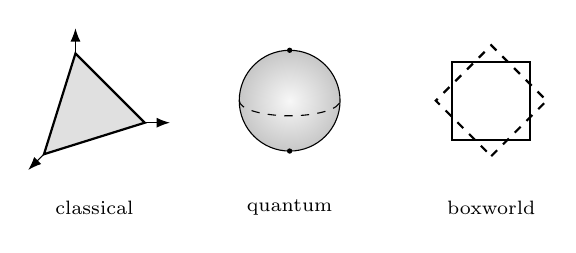
\begin{tikzpicture}[scale=0.8, every node/.style={font=\scriptsize}, >=Latex]
\begin{scope}
\draw[->] (0,0) -- (1.5,0);
\draw[->] (0,0) -- (0,1.5);
\draw[->] (0,0) -- (-0.75,-0.75);
\draw[thick, fill=black!12] (1.1,0) -- (0,1.1) -- (-0.5,-0.5) -- cycle;
\node at (0.3,-1.35) {classical};
\end{scope}
\begin{scope}[xshift=3.4cm]
\shade[inner color=black!3, outer color=black!22] (0,0.35) circle (0.8);
\draw (0,0.35) circle (0.8);
\draw[dashed] (-0.8,0.35) arc (180:360:0.8 and 0.24);
\fill (0,1.15) circle (1.2pt);
\fill (0,-0.45) circle (1.2pt);
\node at (0,-1.35) {quantum};
\end{scope}
\begin{scope}[xshift=6.6cm]
\draw[thick] (-0.62,-0.27) rectangle (0.62,0.97);
\draw[thick, dashed] (0,-0.53) -- (0.88,0.35) -- (0,1.23) -- (-0.88,0.35) -- cycle;
\node at (0,-1.35) {boxworld};
\end{scope}
\end{tikzpicture}
\caption{Normalized-state slices. Classical: simplex (self-dual orthant). Quantum: Bloch ball (self-dual PSD cone). Boxworld: square, dual slice dashed --- not self-dual.}
\label{fig:examples}
\end{figure}

Examples (Fig.~\ref{fig:examples}): classical $(\mathbb{R}^N,\mathbb{R}^N_{\ge0},\textstyle\sum_i)$, quantum $(\mathrm{H}_N(\mathbb{C}),\mathrm{PSD},\operatorname{tr})$, boxworld (cone over the square \cite{Barrett2007}). Self-duality of the state cone is the property that will decide everything below.

\section{One dimension: dualizability}\label{sec:1d}

\begin{itemize}
\item $\mathbf{Bord}_1$: generated by $\operatorname{id}_+$, cup $\cup:\varnothing\to+\sqcup-$, cap $\cap:-\sqcup+\to\varnothing$, modulo the snakes; $S^1=\cap\circ\sigma\circ\cup$. A $1$d theory \emph{is} a dualizable object $X=Z(+)$ \cite{Lurie2009}.
\item In $\mathbf{Vec}$: every object dualizable, $\operatorname{coev}(1)=g:=\sum_af_a\otimes f^a$, snakes $=$ resolution of identity, $Z(S^1)=\dim_{\mathbb R}V$. Classification: one integer. Nothing to check.
\item In GPT: the dual is \emph{forced}, $X^\vee=(V^*,(V^+)^*,u^\vee)$, and dualizability of $X=(V,V^+,u)$ reduces to two memberships of the \emph{single} element $g$:
\begin{align}
\text{cup (state):}&\quad g\in V^+_{X\otimes X^\vee},\label{eq:cup}\\
\text{cap (effect):}&\quad g\in\big(V^+_{X^\vee\otimes X}\big)^{*}.\label{eq:cap}
\end{align}
The cup wants the composite cone large, the cap wants it small; min--max duality exchanges the two ends. Operationally, \eqref{eq:cup}--\eqref{eq:cap} assert exact teleportation with $g$ as both resource and measurement \cite{BBLW}.
\item Conjecture: \eqref{eq:cup}--\eqref{eq:cap} are satisfiable iff $V^+$ is \emph{weakly self-dual}. Classical: passes, $g$ separable ($\in\otimes_{\min}$). Quantum: passes, $g$ $=$ maximally entangled element after a transpose twist. Boxworld: no-go (square cone not self-dual; only finitely many twists).
\item Koecher--Vinberg \cite{KoecherVinberg} $+$ BBLW steering \cite{BBLW}: homogeneous self-dual cones are Euclidean Jordan algebras $\Rightarrow$ theories passing the $1$d test are ``close to quantum.''
\end{itemize}

\section{Two dimensions: the Frobenius data as GPT data}\label{sec:2d}

\begin{figure}[t]
\centering
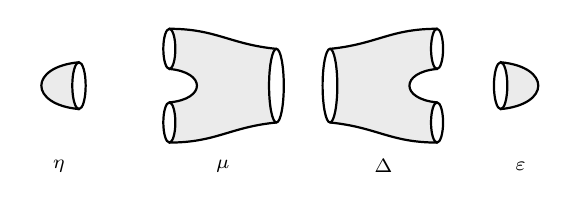
\begin{tikzpicture}[scale=0.85, every node/.style={font=\scriptsize}]
% eta: disk with outgoing circle
\begin{scope}
\fill[black!8] (0.55,0.35) .. controls (-0.2,0.28) and (-0.2,-0.28) .. (0.55,-0.35) arc (-90:90:0.1 and 0.35);
\draw[thick] (0.55,0.35) .. controls (-0.2,0.28) and (-0.2,-0.28) .. (0.55,-0.35);
\draw[thick, fill=white] (0.55,0) ellipse (0.1 and 0.35);
\node at (0.25,-1.2) {$\eta$};
\end{scope}
% mu: pants, two in, one out
\begin{scope}[xshift=1.9cm]
\fill[black!8] (0,0.85) .. controls (0.7,0.85) and (0.9,0.62) .. (1.6,0.55) -- (1.6,-0.55) .. controls (0.9,-0.62) and (0.7,-0.85) .. (0,-0.85) -- (0,-0.25) .. controls (0.55,-0.2) and (0.55,0.2) .. (0,0.25) -- cycle;
\draw[thick] (0,0.85) .. controls (0.7,0.85) and (0.9,0.62) .. (1.6,0.55);
\draw[thick] (0,-0.85) .. controls (0.7,-0.85) and (0.9,-0.62) .. (1.6,-0.55);
\draw[thick] (0,0.25) .. controls (0.55,0.2) and (0.55,-0.2) .. (0,-0.25);
\draw[thick, fill=white] (0,0.55) ellipse (0.09 and 0.3);
\draw[thick, fill=white] (0,-0.55) ellipse (0.09 and 0.3);
\draw[thick, fill=white] (1.6,0) ellipse (0.11 and 0.55);
\node at (0.8,-1.2) {$\mu$};
\end{scope}
% Delta: copants, one in, two out
\begin{scope}[xshift=5.9cm, xscale=-1]
\fill[black!8] (0,0.85) .. controls (0.7,0.85) and (0.9,0.62) .. (1.6,0.55) -- (1.6,-0.55) .. controls (0.9,-0.62) and (0.7,-0.85) .. (0,-0.85) -- (0,-0.25) .. controls (0.55,-0.2) and (0.55,0.2) .. (0,0.25) -- cycle;
\draw[thick] (0,0.85) .. controls (0.7,0.85) and (0.9,0.62) .. (1.6,0.55);
\draw[thick] (0,-0.85) .. controls (0.7,-0.85) and (0.9,-0.62) .. (1.6,-0.55);
\draw[thick] (0,0.25) .. controls (0.55,0.2) and (0.55,-0.2) .. (0,-0.25);
\draw[thick, fill=white] (0,0.55) ellipse (0.09 and 0.3);
\draw[thick, fill=white] (0,-0.55) ellipse (0.09 and 0.3);
\draw[thick, fill=white] (1.6,0) ellipse (0.11 and 0.55);
\node at (0.8,-1.2) {$\Delta$};
\end{scope}
% epsilon: disk with incoming circle
\begin{scope}[xshift=7.4cm, xscale=-1]
\fill[black!8] (0.55,0.35) .. controls (-0.2,0.28) and (-0.2,-0.28) .. (0.55,-0.35) arc (-90:90:0.1 and 0.35);
\draw[thick] (0.55,0.35) .. controls (-0.2,0.28) and (-0.2,-0.28) .. (0.55,-0.35);
\draw[thick, fill=white] (0.55,0) ellipse (0.1 and 0.35);
\node at (0.25,-1.2) {$\varepsilon$};
\end{scope}
\end{tikzpicture}
\caption{Generators of $\mathbf{Bord}_2$: disk $\eta$, pants $\mu$, copants $\Delta$, reversed disk $\varepsilon$ (time flows left to right).}
\label{fig:pants}
\end{figure}

A $2$d theory assigns $X:=Z(S^1)=(V,V^+,u)$ and one morphism per generator (Fig.~\ref{fig:pants}); the relations (unit, counit, (co)associativity, (co)commutativity, Frobenius) are equalities of linear maps, unchanged from $\mathbf{Vec}$. The finite data, read in GPT:

\begin{center}
\renewcommand{\arraystretch}{1.5}
\begin{tabular}{lll}
bordism & algebra & GPT positivity\\
\hline
disk $\eta:\varnothing\to S^1$ & unit $1_A$ & a state: $\eta(1)\in V^+$\\
rev.\ disk $\varepsilon:S^1\to\varnothing$ & counit & an effect: $\varepsilon\in(V^+)^*$\\
pants $\mu:S^1\sqcup S^1\to S^1$ & product & $\mu\big(V^+_{XX}\big)\subseteq V^+$\\
copants $\Delta:S^1\to S^1\sqcup S^1$ & coproduct & $\Delta\big(V^+\big)\subseteq V^+_{XX}$
\end{tabular}
\end{center}

\begin{defi}[$2$d GPTFT, finite data]
A GPT system $X=(V,V^+,u)$, a composite cone $V^+_{XX}\in[\otimes_{\min},\otimes_{\max}]$, and four \emph{positive} structure maps $\eta,\varepsilon,\mu,\Delta$ as in the table, satisfying the (co)unit, (co)associativity, (co)commutativity and Frobenius relations. Equivalently: a commutative Frobenius algebra in $\mathbf{Vec}$ all of whose structure maps are positive for the chosen cones.
\end{defi}

\paragraph{Conceptual points.}
\begin{itemize}
\item \emph{Operational reading.} The unit is a preparation (a distinguished unnormalized state created by the disk); the counit is a measurement outcome; merging ($\mu$) and splitting ($\Delta$) of circles are physical transformations.
\item \emph{The cone tension returns.} $\mu$ is easiest to make positive when $V^+_{XX}$ is \emph{small} (fewer inputs to control), $\Delta$ when it is \emph{large} (more room for outputs): the $2$d incarnation of the $1$d cup/cap tension, now on genuinely independent data.
\item \emph{The $1$d problem embeds.} The derived pairing and copairing
\[
\beta:=\varepsilon\circ\mu\in\big(V^+_{XX}\big)^*,\qquad
\gamma:=\Delta(\eta(1))\in V^+_{XX}
\]
are a positive effect and a positive state, and the Frobenius $+$ (co)unit relations force the snake identities for $(\gamma,\beta)$. Hence $X$ is dualizable with $X^\vee\cong X$: the $2$d structure contains a solution of the $1$d problem \emph{with the dual identified with the object itself}.
\item \emph{Self-duality becomes necessary.} Since the dual is forced to be $X^\vee=(V^*,(V^+)^*,u^\vee)$, the isomorphism $X\cong X^\vee$ is a positive linear isomorphism $V\cong V^*$ carrying $V^+$ onto $(V^+)^*$: \emph{weak self-duality of the state cone is a necessary condition for a $2$d GPTFT}. What is conjectural in $1$d is forced in $2$d. Immediate corollary: boxworld admits no $2$d GPTFT.
\item \emph{Invariants are nonnegative.} The handle operator $h:=\mu\circ\Delta$ is a positive endomorphism of $X$, and
\[
Z(\Sigma_g)=\varepsilon\big(h^g(\eta(1))\big)\ \ge\ 0 :
\]
every closed surface evaluates to a composition of positive data --- an (unnormalized) probability. In particular $Z(S^2)=\varepsilon(\eta(1))\ge0$ and $Z(T^2)=\dim_{\mathbb R}V$.
\item \emph{Classical example passes.} $V=\mathbb{R}^N$ with the pointwise algebra: $\eta(1)=\sum_ie_i$, $\varepsilon(e_i)=\lambda_i>0$, $\mu(e_i\otimes e_j)=\delta_{ij}e_i$, $\Delta(e_i)=\lambda_i^{-1}\,e_i\otimes e_i$. All four maps are positive (for the unique classical composite cone, $\otimes_{\min}=\otimes_{\max}$), $\beta$ is nondegenerate: classical $2$d GPTFTs exist, one family per choice of weights $\lambda$.
\item \emph{Quantum is the open case.} The PSD cone passes the necessary self-duality condition, but the obvious products fail: matrix multiplication is neither commutative nor Hermiticity-preserving; the Jordan product is commutative but not associative. Whether $\mathrm{H}_N(\mathbb{C})$ ($N\ge2$) carries \emph{some} commutative, associative, positive Frobenius structure --- and more generally, which weakly self-dual cones do --- is the $2$d classification problem.
\end{itemize}

\begin{thebibliography}{99}

\bibitem{Atiyah1988}
M.~F.~Atiyah,
\emph{Topological quantum field theories},
Publ.\ Math.\ IH\'ES \textbf{68}, 175 (1988).

\bibitem{Segal2004}
G.~Segal,
\emph{The definition of conformal field theory},
in \emph{Topology, Geometry and Quantum Field Theory},
London Math.\ Soc.\ Lecture Note Ser.\ \textbf{308}
(Cambridge University Press, 2004).

\bibitem{Hardy2001}
L.~Hardy,
\emph{Quantum theory from five reasonable axioms},
arXiv:quant-ph/0101012.

\bibitem{Barrett2007}
J.~Barrett,
\emph{Information processing in generalized probabilistic theories},
Phys.\ Rev.\ A \textbf{75}, 032304 (2007),
arXiv:quant-ph/0508211.

\bibitem{Mueller2021}
M.~P.~M\"uller,
\emph{Probabilistic theories and reconstructions of quantum theory},
SciPost Phys.\ Lect.\ Notes \textbf{28} (2021),
arXiv:2011.01286.

\bibitem{Plavala2023}
M.~Pl\'avala,
\emph{General probabilistic theories: An introduction},
Phys.\ Rep.\ \textbf{1033}, 1 (2023),
arXiv:2103.07469.

\bibitem{ALPP2021}
G.~Aubrun, L.~Lami, C.~Palazuelos, and M.~Pl\'avala,
\emph{Entangleability of cones},
Geom.\ Funct.\ Anal.\ \textbf{31}, 181 (2021),
arXiv:1911.09663.

\bibitem{Lurie2009}
J.~Lurie,
\emph{On the classification of topological field theories},
Current Developments in Mathematics \textbf{2008}, 129 (Int.\ Press, 2009),
arXiv:0905.0465.

\bibitem{BBLW}
H.~Barnum, J.~Barrett, M.~Leifer, and A.~Wilce,
\emph{Teleportation in general probabilistic theories},
Proc.\ Sympos.\ Appl.\ Math.\ (AMS, 2012),
arXiv:0805.3553.

\bibitem{KoecherVinberg}
M.~Koecher, \emph{The Minnesota Notes on Jordan Algebras and Their Applications},
Lecture Notes in Mathematics \textbf{1710} (Springer, 1999);
E.~B.~Vinberg, \emph{The theory of convex homogeneous cones},
Trans.\ Moscow Math.\ Soc.\ \textbf{12}, 340 (1963).

\bibitem{Dijkgraaf1989}
R.~Dijkgraaf,
\emph{A geometrical approach to two-dimensional conformal field theory},
Ph.D.\ thesis, Utrecht University (1989).

\bibitem{Abrams1996}
L.~Abrams,
\emph{Two-dimensional topological quantum field theories and Frobenius algebras},
J.\ Knot Theory Ramifications \textbf{5}, 569 (1996).

\bibitem{Kock2004}
J.~Kock,
\emph{Frobenius Algebras and 2D Topological Quantum Field Theories},
London Math.\ Soc.\ Student Texts \textbf{59}
(Cambridge University Press, 2004).

\end{thebibliography}

\end{document}
